%%%%%%%%%%%%%%%%%%%%%%%%%%%%%%%%%%%%%%%%%%%%%%%%%%%%%%%%%%%%
%%  This Beamer template was created by Cameron Bracken.
%%  Anyone can freely use or modify it for any purpose
%%  without attribution.
%%
%%  Last Modified: January 9, 2009
%%

\documentclass[xcolor=x11names,compress]{beamer}

%% General document %%%%%%%%%%%%%%%%%%%%%%%%%%%%%%%%%%
\usepackage{graphicx}
\usepackage{tikz}
\usepackage[utf8]{inputenc}
\usepackage[spanish]{babel}
\usetikzlibrary{decorations.fractals}
%%%%%%%%%%%%%%%%%%%%%%%%%%%%%%%%%%%%%%%%%%%%%%%%%%%%%%


%% Beamer Layout %%%%%%%%%%%%%%%%%%%%%%%%%%%%%%%%%%
\useoutertheme[subsection=false,shadow]{miniframes}
\useinnertheme{default}
\usefonttheme{serif}
\usepackage{palatino}
\DeclareUnicodeCharacter{00A0}{ }

\setbeamerfont{title like}{shape=\scshape}
\setbeamerfont{frametitle}{shape=\scshape}

\setbeamercolor*{lower separation line head}{bg=DeepSkyBlue4} 
\setbeamercolor*{normal text}{fg=black,bg=white} 
\setbeamercolor*{alerted text}{fg=red} 
\setbeamercolor*{example text}{fg=black} 
\setbeamercolor*{structure}{fg=black} 
 
\setbeamercolor*{palette tertiary}{fg=black,bg=black!10} 
\setbeamercolor*{palette quaternary}{fg=black,bg=black!10} 

\renewcommand{\(}{\begin{columns}}
\renewcommand{\)}{\end{columns}}
\newcommand{\<}[1]{\begin{column}{#1}}
\renewcommand{\>}{\end{column}}
%%%%%%%%%%%%%%%%%%%%%%%%%%%%%%%%%%%%%%%%%%%%%%%%%%




\begin{document}


\begin{frame}
\title{Divide y discriminarás:\\ Una versión distribuída de discriminación de sentidos}
\author{
	Ezequiel Torti López\\}
\subject{Procesamiento de Lenguaje Natural}
\institute{Facultad de Matemática, Astronomía y Física\\Universidad Nacional de Córdoba}
\date{

	\today
}
\titlepage
\end{frame}
%%%%%%%%%%%%%%%%%%%%%%%%%%%%%%%%%%%%%%%%%%%%%%%%%%%%%%
%%%%%%%%%%%%%%%%%%%%%%%%%%%%%%%%%%%%%%%%%%%%%%%%%%%%%%
\section{\scshape Introducción}
%%%%%%%%%%%%%%%%%%%%%%%%%%%%%%%%%%%%%%%%%%%%%%%%%%%%%%
%%%%%%%%%%%%%%%%%%%%%%%%%%%%%%%%%%%%%%%%%%%%%%%%%%%%%%
\subsection{Introducción}
\begin{frame}{Introducción}
\begin{itemize}
\item Disambiguación de palabras: asignación de sentidos a palabras.
\item Dos subproblemas:
\begin{itemize}
\item Sense discrimination
\item Sense labeling
\end{itemize}
\item Nos concentraremos en Sense discrimination.
\end{itemize}
\end{frame}
%%%%%%%%%%%%%%%%%%%%%%%%%%%%%%%%%%%%%%%%%%%%%%%%%%%%%%
%%%%%%%%%%%%%%%%%%%%%%%%%%%%%%%%%%%%%%%%%%%%%%%%%%%%%%
\subsection{Introducción}
\begin{frame}{Introducción}
\begin{itemize}
\item Trataré de reproducir el algoritmo de context-group discrimination (Shütze, 1998)
\item Implementa Sense discrimination. No depende de fuentes de conocimiento externas.
\item Aplicaciones:
\begin{itemize}
\item Para algunos problemas de Information Access, sólo es necesario discriminar sentidos.
\item Ej: Similitud y ranking de documentos; dar ejemplos de sentidos de una palabra para una query ambigua.
\end{itemize}
\end{itemize}
\end{frame}
%%%%%%%%%%%%%%%%%%%%%%%%%%%%%%%%%%%%%%%%%%%%%%%%%%%%%%
%%%%%%%%%%%%%%%%%%%%%%%%%%%%%%%%%%%%%%%%%%%%%%%%%%%%%%
\subsection{Introducción}
\begin{frame}{Introducción}
\begin{itemize}
\item La implementación será sobre un sistema distribuído utilizando Hadoop.
\item ¿Por qué?
\begin{itemize}
\item Buscar una forma de procesar grandes cantidades de datos (hablamos de TB).
\item Hacerlo de forma rápida.
\item Hadoop puede ser útil para algunas cosas \em{si se usa bien}.
\end{itemize}
%Acá hablar sobre que no tengo un corpus de 5 TB, pero dejo sentada una base por si algun dia lo tuviera.
\end{itemize}
\end{frame}

%%%%%%%%%%%%%%%%%%%%%%%%%%%%%%%%%%%%%%%%%%%%%%%%%%%%%%
%%%%%%%%%%%%%%%%%%%%%%%%%%%%%%%%%%%%%%%%%%%%%%%%%%%%%%
\section{\scshape Context-Group}
\subsection{Context-Group Discrimination}


\begin{frame}{Context-Group Discrimination}
\begin{itemize}
\item Idea:
\begin{itemize}
\item Inducir sentidos de palabras por las similitudes de los contextos en los que ocurren.
\item La similitud contextual incluso juega un papel crucial en categorización semántica que hacen los humanos.
\end{itemize}
\item Ejemplo:
\begin{itemize}
\item \em Tenía un vaso de asdf en la mano.\em
\item \em Se le cayó la botella de asdf al piso. \em
\item \em Tomó tanto asdf que al final no podía caminar.\em
\end{itemize}
\item ¿Qué es \em adsf\em?
\end{itemize}
\end{frame}

\begin{frame}{Context-Group Discrimination}
\begin{itemize}
\item Idea:
\begin{itemize}
\item Agrupar ocurrencias de palabras en clusters.
\item Cada cluster consiste en palabras con contextos similares.
\item Palabras, contextos y sentidos son representados en un espacio vectorial.
\item Para armar Word Vectors, se observan las coocurrencias de una palabra en una ventana de 50 palabras.
\item Para Context Vectors, se observarán coocurrencias de segundo orden (robustez).
\item Para Sense Vectors, se aglomeran los Context Vectors en clusters y se obtienen sus centroides.
\end{itemize}
\end{itemize}
\end{frame}


\begin{frame}{Context-Group Discrimination}
¿Cómo funciona?
\begin{figure}
\centering
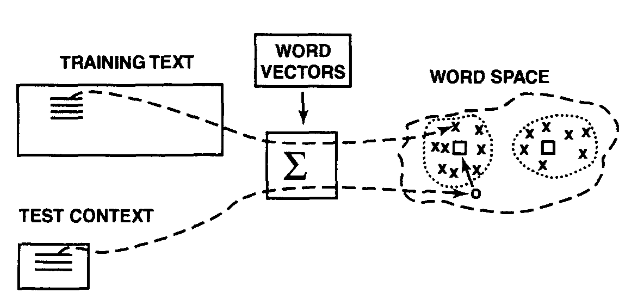
\includegraphics[scale=0.5, keepaspectratio=True, natwidth=800,natheight=600]{basig_design.png}
\end{figure}
\end{frame}

%%%%%%%%%%%%%%%%%%%%%%%%%%%%%%%%%%%%%%%%%%%%%%%%%%%%%%
%%%%%%%%%%%%%%%%%%%%%%%%%%%%%%%%%%%%%%%%%%%%%%%%%%%%%%
\subsection{Word Vectors}
\begin{frame}{Word Vectors}
\begin{itemize}
\item Un Word Vector se construye con los \em n \em vecinos de una palabra en el corpus.
\item Una celda \em i \em en el vector representa \# veces de coocurrencia de la palabra con la palabra en la posición \em i\em.
\item Mientras más overlap haya entre dos vectores, más similiares serán las palabras que representan.
\item ¿Qué palabras usar como dimensiones? Elección: elegir las palabras más frecuentes en el corpus.
\end{itemize}
\begin{figure}
\centering
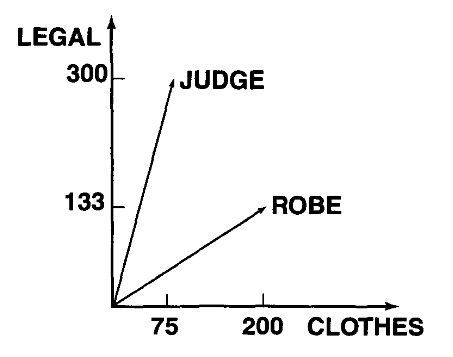
\includegraphics[scale=0.24, keepaspectratio=True, natwidth=800,natheight=600]{word_vector.png}
\end{figure}
\end{frame}

%%%%%%%%%%%%%%%%%%%%%%%%%%%%%%%%%%%%%%%%%%%%%%%%%%%%%%
%%%%%%%%%%%%%%%%%%%%%%%%%%%%%%%%%%%%%%%%%%%%%%%%%%%%%%
\subsection{Context Vectors}
\begin{frame}{Context Vectors}
\begin{itemize}
\item Los WV mezclan sentidos en un solo vector.
\item Necesitamos recorrer el corpus nuevamente, pero esta vez:
\begin{itemize}
\item Analizamos el contexto individual de cada palabra.
\item Sumamos los Word Vectors de las palabras que coocurren = Context Vectors
\end{itemize}
\item Es decir, un Context Vector es un centroide (o suma) de las palabras que ocurren en un contexto.
\end{itemize}
\begin{figure}
\centering
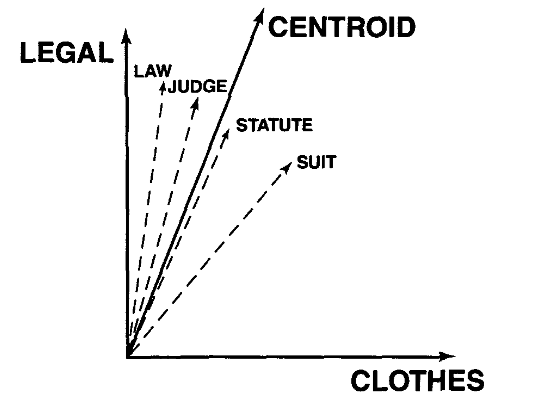
\includegraphics[scale=0.24, keepaspectratio=True, natwidth=800,natheight=600]{context_vector.png}
\end{figure}
\end{frame}

%%%%%%%%%%%%%%%%%%%%%%%%%%%%%%%%%%%%%%%%%%%%%%%%%%%%%%
%%%%%%%%%%%%%%%%%%%%%%%%%%%%%%%%%%%%%%%%%%%%%%%%%%%%%%
\subsection{Sense Vectors}
\begin{frame}{Sense Vectors}
\begin{itemize}
\item Son grupos de contextos similares.
\item Se arman clusters partiendo de TODOS los contextos analizados en el corpus.
\item Un Sense Vector es simplemente un centroide de cada uno de esos clusters.
\item Para armar los clusters se utiliza EM.
\begin{itemize}
\item Puede converger a soluciones óptimas locales.
\item Es necesario elegir buenos parámetros iniciales, sino puede converger a mínimos locales.
\item Alternativa: Usar Group-Average agglomerative clustering (GAAC).
\end{itemize}
\end{itemize}
\end{frame}

\subsection{Sense Vectors}
\begin{frame}{Sense Vectors}
\begin{itemize}
\item El resultado del clustering depende de la representación de los Context Vectors.
\begin{itemize}
\item Se utiliza una transformación del espacio dimensional (Singular Value Descomposition).
\item SVD encuentra los ejes de mayor variación en el espacio vectorial.
\item Se representan los Context vectors utilizando solamente estas dimensiones.
\item Se obtienen mejores mediciones que con los vectores sin reducir.
\end{itemize}
\end{itemize}
\begin{figure}
\centering
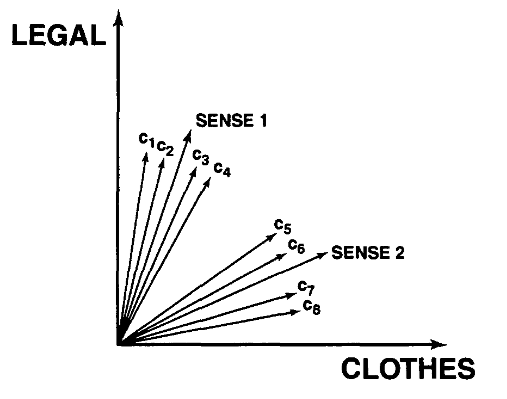
\includegraphics[scale=0.24, keepaspectratio=True, natwidth=800,natheight=600]{sense_vector.png}
\end{figure}
\end{frame}


\begin{frame}{Context-Group Discrimination}
Finalmente...\\
Para discriminar una ocurrencia \em T \em de una palabra ambigua \em V \em:
\begin{itemize}
\item Mapear \em T \em en su correspondiente Context Vector $\vec c$ usando los WV de las palabras de su contexto.
\item Obtener los Sense Vectors $\vec S_j$ de \em V \em.
\item Asignar \em T \em al sentido \em j \em cuyo Sense Vector es más cercano a $\vec c$.
\end{itemize}
\end{frame}


%%%%%%%%%%%%%%%%%%%%%%%%%%%%%%%%%%%%%%%%%%%%%%%%%%%%%%
%%%%%%%%%%%%%%%%%%%%%%%%%%%%%%%%%%%%%%%%%%%%%%%%%%%%%%
\section{\scshape Variantes}
\subsection{Variantes}
\begin{frame}{Variantes}
\begin{itemize}
\item Se utilizó el Wiki Corpus en español.
\item Se preprocesó el corpus para dejarlo en forma de lemmas. Esto facilitó el trabajo posterior.
\item El algoritmo se implementa usando Hadoop. Se busca de esta forma sentar una base a lo que es el procesamiento de grandes cantidades de datos.
\end{itemize}
\end{frame}


%%%%%%%%%%%%%%%%%%%%%%%%%%%%%%%%%%%%%%%%%%%%%%%%%%%%%%
%%%%%%%%%%%%%%%%%%%%%%%%%%%%%%%%%%%%%%%%%%%%%%%%%%%%%%
\section{\scshape Hadoop+Dumbo}
\subsection{Hadoop}
\begin{frame}{Introducción a Hadoop}
\begin{itemize}
\item Es un Framework para aplicaciones distribuídas.
\item Principalmente proceso de datos a larga escala.
\item Cuenta con varios módulos:
\begin{itemize}
\item Un sistema de archivos distribuídos (HDFS).
\item Librerías en común.
\item Plataforma de manejo de recursos.
\item MapReduce: Un modelo de programación para procesamiento de datos.
\end{itemize}
\end{itemize}
\end{frame}

\begin{frame}{Mapreduce}
Definir dos funciones:
\begin{itemize}
\item Map: toma un valor y devuelve un par (\em key:value\em).
\begin{itemize}
\item No requiere estado, por lo tanto es ejecutable en paralelo.
\item Ej: toma una palabra, y devuelve la longitud (\em key\em) y la palabra misma (\em value\em)
\end{itemize}
\item El framework se encarga de agrupar valores con las mismas \em keys\em.
\item Reduce: toma (\em key:list\_of\_values \em). Devuelve otro par (\em key:value\em).
\begin{itemize}
\item Ej: toma un número (\em key \em) y una lista de palabras con esa longitud (\em list\_of\_values\em).
\item Ej: podría devolver \em key \em y la cantidad de palabras en \em list\_of\_values \em.
\end{itemize}
\end{itemize}
\end{frame}


\begin{frame}{Mapreduce}
\begin{figure}
\centering
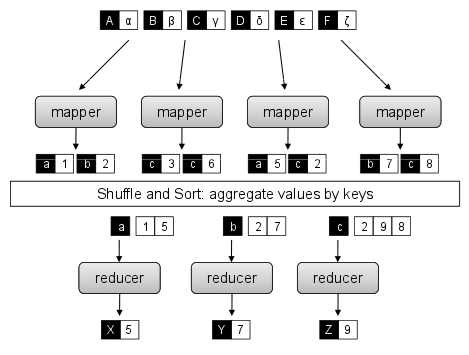
\includegraphics[scale=0.5, keepaspectratio=True, natwidth=800,natheight=600]{mapreduce.png}
\end{figure}
\end{frame}


\begin{frame}{Dumbo}
\begin{itemize}
\item MapReduce $\rightarrow$ Java. Pero soporta streaming.
\item Podemos usar cualquier lenguaje, siempre que lea y escriba en stdin/stdout.
\item Dumbo: Módulo Python, una especie de API para escribir programas para Hadoop sobre Python.
\end{itemize}
\end{frame}


%%%%%%%%%%%%%%%%%%%%%%%%%%%%%%%%%%%%%%%%%%%%%%%%%%%%%%
%%%%%%%%%%%%%%%%%%%%%%%%%%%%%%%%%%%%%%%%%%%%%%%%%%%%%%
\section{\scshape Implementación}
\subsection{Paso 0}
\begin{frame}{Paso 0: Preprocesamiento}
\begin{itemize}
\item Pequeño programa en C++ para transformar corpus.
\item Razón: Lento y costoso levantar instancia de Freeling en cada Map.
\item Al no tener un cluster real, facilita las tareas en los pasos siguientes.
\end{itemize}
\end{frame}

\subsection{Paso 1}
\begin{frame}{Paso 1: Contar Palabras}
\begin{itemize}
\item Simple programa MapReduce para contar las ocurrencias de palabras en el corpus.
\item Se obtienen las 20000 palabras más frecuentes del corpus para analizar.
\item las primeras 2000 serán usadas como dimensiones también.
\end{itemize}
\end{frame}

\subsection{Paso 2}
\begin{frame}{Paso 2: Contar Coocurrencias}
\begin{itemize}
\item Armar Word Vectors en una ventana de 50 palabras
\item Input: corpus y un archivo que contiene la lista de palabras a analizar.
\item Las primeras 2000 palabras serán las dimensiones.
\item Output:
\begin{itemize}
\item[Opción 1] por cada coocurrencia, devolver par \em palabra:coocurrencia\em.
\item[Opción 2] por cada palabra analizada, devolver diccionario de coocurrencias.
\end{itemize}
\end{itemize}
\end{frame}


\subsection{Paso 3}
\begin{frame}{Paso 3: Calcular SVD}
\begin{itemize}
\item Sin usar Hadoop.
\item Se reducen las dimensiones de los WV de 2000 a 100.
\end{itemize}
\end{frame}


\subsection{Paso 4}
\begin{frame}{Paso 4: Armar Context Vectors}
\begin{itemize}
\item Input: corpus, matriz de coocurrencias.
\item Se vuelve a recorrer el corpus.
\item Arma los Context Vector de cada ocurrencia de una palabra, sumando los Word Vectors de las palabras con las que coocurre.
\end{itemize}
\end{frame}


\subsection{Paso 5}
\begin{frame}{Paso 4: Armar Clusters de Context Vectors}
\begin{itemize}
\item Input: Context Vectors.
\item Se aglomeran en clusters.
\item Los centroides de los Clusters son los Sense Vectors.
\item Guardar esa información $\rightarrow$ Discriminar nuevas palabras por contexto.
\end{itemize}
\end{frame}


%%%%%%%%%%%%%%%%%%%%%%%%%%%%%%%%%%%%%%%%%%%%%%%%%%%%%%
%%%%%%%%%%%%%%%%%%%%%%%%%%%%%%%%%%%%%%%%%%%%%%%%%%%%%%
\section{\scshape Bottlenecks}
\subsection{Bottlenecks}
\begin{frame}{Bottlenecks}
\begin{itemize}
\item Alta tasa de transmisión de datos $\rightarrow$ Muchos paquetes en la red
\begin{itemize}
\item Solución: evitar mandar tantos paquetes.
\end{itemize}
\item Mal balance de carga en cada nodo $\rightarrow$ Maps más lentos que otros.
\begin{itemize}
\item En algunos pasos, evitar analizar palabras con poco poder de discriminación y que son muy frecuentes.
\end{itemize}
\item Evitar uso de tantas librerías externas: Freeling.
\end{itemize}
\end{frame}

%%%%%%%%%%%%%%%%%%%%%%%%%%%%%%%%%%%%%%%%%%%%%%%%%%%%%%
%%%%%%%%%%%%%%%%%%%%%%%%%%%%%%%%%%%%%%%%%%%%%%%%%%%%%%
\section{\scshape Eval}
\subsection{Evaluación}
\begin{frame}{Evaluación}
\begin{itemize}
\item Ideas:
\begin{itemize}
\item Evaluar los datos obtenidos sobre un grupo reducido de palabras del lenguaje natural.
\item Comparar resultados con los datos originales clasificados manualmente.
\item Evaluar distintas formas de hacer clustering: K-means, GAAC.
\item Si todo va bien, evaluar con palabras artificiales (\em bananadoor \em).
\end{itemize}
\end{itemize}
\end{frame}

\end{document}
